\chapter{Elecciones UNComa con Gukena}
\label{Gukena2}
El proceso electoral comienza cuando se definen las fechas de oficialización de padrones y listas, acto electoral, escrutinio provisorio, escrutinio definitivo y proclamación de autoridades electas. Se considera que un sistema de votación exitoso debe cumplir el principal objetivo que es construir la confianza de toda persona involucrada en el proceso. 
Antes del 2015, una única persona era responsable de gestionar correctamente los resultados y distribuir los cargos. La forma de trabajo generaba un cuello de botella en la carga de los datos y una demora de varias horas y hasta días en obtener los resultados finales. \newline
A continuación se detallan los resultados obtenidos luego de comenzar a utilizar Gukena en las elecciones de la universidad agrupados por año. Estas experiencias brindaron un gran aporte a esta tesis al poder analizar la implementación de este sistema en un contexto real.

\section{Experiencia 16 de Junio de 2015}
Para las elecciones celebradas el 16 de Junio de 2015, Gukena se validó con el archivo xls usado en el escrutinio. Este año tuvo información de 18 Unidades Electorales distribuidas en 16 localidades con un total de 34 mesas. 
Ese año, la Universidad renovó integrantes del Consejo Directivo de cada unidad académica y del Consejo Superior de la Universidad, para el claustro de Estudiantes.

De este modo, el sistema se puso a prueba frente a la siguiente información:
\begin{itemize}
    \item La Elección se desarrolló en 18 Unidades Electorales repartidas en 34 Sedes.
    \item 34 mesas distribuidas en las distintas sedes
    \item 9.560 empadronados del claustro Estudiantes
    \item 9 listas para el Consejo Superior
    \item 45 listas para el Consejo Directivo distribuidas entre las diferentes sedes y asentamientos
\end{itemize}
A pesar de que este año no se utilizó el sistema durante el escrutinio, los datos se encuentran disponible en las elecciones históricas presente en la página de Resultados de Gukena.

\section{Experiencia 14 al 17 de Mayo de 2016}
\label{exp2016}
Primera vez que el sistema se integró al proceso electoral de la universidad para las elecciones celebradas desde el 14 al 17 de Mayo de 2016. Gukena contó con información de 18 Unidades Electorales distribuidas en 16 localidades con un total de 77 mesas. 
Ese año, la Universidad renovó integrantes del Consejo Directivo de cada unidad académica y del Consejo Superior de la Universidad, para los claustros de Estudiantes, No Docentes y Graduados. 

De este modo, el sistema operó frente a la siguiente información:
\begin{itemize}
    \item La Elección se desarrolla en 18 Unidades Electorales repartidas en 34 Sedes.
    \item De las 77 mesas distribuidas en las distintas sedes, 18 son para el claustro No docente, 33 son para el claustro Estudiantes y 26 son para el claustro Graduados.
    \item De 22.313 empadronados: 719 son No docentes, 8199 son Estudiantes y 13.395 son Graduados. 
    \item 15 listas para el Consejo Superior, donde 4 son de No docentes, 8 son de Estudiantes y 3 de Graduados.
    \item 121 listas para el Consejo Directivo distribuidas entre las diferentes sedes, asentamientos y distintos claustros.
\end{itemize}

Durante el período de escrutinio, la primer mesa cargada con éxito en el sistema fue la Facultad de Ciencias y Ambientes de la Salud, para el claustro de graduados, 5 minutos después del cierre.\\ 
Con la utilización del sistema, se obtuvo la siguiente información estadística:
66 mesas fueron cargadas directamente por autoridades de mesas siendo el 86\% del total, 39 mesas fueron cargadas entre las 20:00 hs y 21:56 hs, siendo el 51\% del total.\\
11 mesas fueron cargados por la junta electoral, de las cuales una fue corregida en una segunda etapa de verificación.
Sólo 3 valores de actas fueron corregidas por la Junta Electoral, lo que implica un 0,3\% de error en lo cargado por las autoridades de mesa, o lo que es lo mismo un 99,7\% de datos correctos cargados por las autoridades de mesas.

Las razones por las cuales 11 actas no pudieron ser cargadas por las Autoridades de Mesa son las siguientes:
\begin{itemize}
\item La persona destinada a cargar los datos no contaba con experiencia en el uso de la computadora.
\item El extravío del sobre que contenía datos de usuario y contraseña enviado junto a la urna.
\item Problemas con la conexión a Internet.
\end{itemize}

\section{Experiencia 13 al 16 de Mayo de 2017}
Gukena procesó información de 17 Unidades Electorales distribuidas en 14 localidades con un total de 32 mesas. Este año, la Universidad renovó integrantes del Consejo Directivo de cada Unidad Académica y el Consejo Superior en el claustro Estudiantes.

De este modo, el sistema operó frente a la siguiente información:
\begin{itemize}
    \item 32 mesas distribuidas en las distintas sedes
    \item El padrón fue de 9504 estudiantes.
    \item 8 listas para Consejo Superior.
    \item 38 listas para el Consejo Directivo entre las diferentes sedes y asentamientos.
\end{itemize}
  
Del total de mesas se tuvo que 31 mesas fueron cargadas por las autoridades de mesa desde la sede donde se realizó la elección y 1 fue cargada por la Junta Electoral. Todos los datos fueron correctamente cargados, esto quiere decir que ningún dato contenido en las actas debió ser corregido por la Junta Electoral, ni por la Secretaria de la misma.
Durante el período de escrutinio, la primer mesa cargada con éxito en el sistema fue la Facultad de Turismo sede San Martín de los Andes, 3 minutos después del cierre.

De la utilización del sistema, se obtuvo la siguiente información estadística:
31 mesas fueron cargadas directamente por autoridades de mesas, siendo el 97\% del total.

Del total de mesas:
15 mesas fueron cargadas entre las 20:00 hs y 21:20 hs, siendo el 47\%,
%20 mesas fueron cargadas entre las 20:00 hs y 21:40 hs, siendo el 63\%,
%22 mesas fueron cargadas entre las 20:00 hs y 21:50 hs, siendo el 69\% y 
%6 mesas fueron cargadas al día siguiente, siendo el 19\%.
1 mesa fue cargada 	por la Junta Electoral, siendo el 3\% del total.

Ningún acta fue corregida por la Junta Electoral, lo que implica un 0\% de error en la carga realizada por las autoridades de mesa, o lo que es lo mismo un 100\% de datos correctamente cargados por las autoridades de mesas.

\section{Experiencia 2018}
\subsection{Primer vuelta 21 al 22 de Mayo de 2018}
Gukena procesó información de 18 Unidades Electorales distribuidas en 14 localidades con un total de 95 mesas. Este año, la universidad renovó integrantes del Rectorado, Decanato, Consejo Directivo de cada unidad y el Consejo Superior de la UNComa en el claustro Estudiantes, Graduados, No Docentes y Docentes.

De este modo, el sistema operó frente a la siguiente información:
\begin{itemize}
    \item 95 mesas distribuidas en las distintas sedes 
     \item El padrón fue de  30192, distribuidos en 9486 estudiantes, 17481 graduados, 718 no docentes y 2507 docentes.
     \item 5 listas para Rectorado.
     \item 30 listas para Decano
    \item 23 listas para Consejo Superior, distribuidos en 7 del claustro Estudiantes, 5 de Graduado, 5 No Docente, 6 Docente.
    \item 133 listas para el Consejo Directivo: 35 del Claustro Estudiantes, 31 de Graduados, 23 No Docentes, 44 Docentes.
\end{itemize}
Del total de mesas, 94 mesas fueron cargadas por las autoridades de mesa desde la sede donde se realizó la elección y 1 fue cargada por la Junta Electoral, 90 mesas fueron correctamente cargados, esto quiere decir que 5 mesas debieron ser corregidos por la Junta Electoral o por la Secretaria de la misma.

Durante el período de escrutinio, la primer mesa cargada con éxito en el sistema fue la unidad electoral AUZA sede Zapala a las 19:38 hrs. debido a que al ser una mesa con muy poca concurrencia se habilitó la carga minutos antes de las 20:00 hrs.

De la utilización del sistema, se obtuvo la siguiente información estadística:
93 mesas fueron cargadas directamente por autoridades de mesas, siendo el 99\% del total.

Del total de mesas:
45 mesas fueron cargadas antes de las 21:30 hs, siendo el 47\%,
%20 mesas fueron cargadas entre las 20:00 hs y 21:40 hs, siendo el 63\%,
%22 mesas fueron cargadas entre las 20:00 hs y 21:50 hs, siendo el 69\% y 
%6 mesas fueron cargadas al día siguiente, siendo el 19\%.
1 mesa fue cargada 	por la Junta Electoral, siendo el 1\% del total.

5 actas fueron corregidas por la Junta Electoral, lo que implica un 5\% de error en la carga realizada por las autoridades de mesa, o lo que es lo mismo un 95\% de datos correctamente cargados por las autoridades de mesas.

\subsection{Segunda vuelta 4 al 5 de Junio de 2018}
Gukena procesó información de 18 Unidades Electorales distribuidas en 14 localidades con un total de 97 mesas. En esta segunda vuelta, la universidad disputó el Rectorado participando los claustros Estudiantes, Graduados, No Docentes y Docentes.

De este modo, el sistema operó frente a la siguiente información:
\begin{itemize}
    \item 97 mesas distribuidas en 26 de las 34 Sedes de la UNComa.
     \item El padrón fue de  30192, distribuidos en 9486 estudiantes, 17481 graduados, 718 no docentes y 2507 docentes.
     \item 5 listas para Rectorado.
\end{itemize}
Del total de mesas, 96 mesas fueron cargadas por las autoridades de mesa desde la sede donde se realizó la elección y 1 fue cargada por la Junta Electoral y, 97 mesas fueron correctamente cargados, esto quiere decir que ninguna mesa debió ser corregida por la Junta Electoral o por la Secretaria de la misma.

Durante el período de escrutinio, la primer mesa cargada con éxito en el sistema fue la unidad electoral ASMA sede San Martin de los Andes a las 20:02 hrs.

De la utilización del sistema, se obtuvo la siguiente información estadística:
96 mesas fueron cargadas directamente por autoridades de mesas, siendo el 99\% del total.

Del total de mesas:
50 mesas fueron cargadas antes de las 20:40 hs, siendo el 52\%,
%20 mesas fueron cargadas entre las 20:00 hs y 21:40 hs, siendo el 63\%,
%22 mesas fueron cargadas entre las 20:00 hs y 21:50 hs, siendo el 69\% y 
%6 mesas fueron cargadas al día siguiente, siendo el 19\%.
1 mesa fue cargada 	por la Junta Electoral, siendo el 1\% del total.

Ningún acta fue corregida por la Junta Electoral, lo que implica un 0\% de error en la carga realizada por las autoridades de mesa, o lo que es lo mismo un 100\% de datos correctamente cargados por las autoridades de mesas.

\section{Experiencia 14 de Mayo de 2019}
Gukena procesó información de 18 Unidades Electorales distribuidas en 14 localidades con un total de 30 mesas. Este año, la Universidad renovó integrantes del Consejo Directivo de cada Unidad Académica y el Consejo Superior en el claustro Estudiantes.

De este modo, el sistema operó frente a la siguiente información:
\begin{itemize}
    \item 30 mesas distribuidas en las distintas sedes
     \item El padrón fue de  9283 estudiantes.
     \item 27 listas para el Consejo Directivo del Claustro Estudiantes.
     \item 7 listas para Consejo Superior
\end{itemize}
Del total de mesas, 30 mesas fueron cargadas por las autoridades de mesa desde la sede donde se realizó la elección y ninguna mesa fue cargada por la Junta Electoral y, ninguna mesa debió ser corregida por la Junta Electoral o por la Secretaria de la misma.

Durante el período de escrutinio, la primer mesa cargada con éxito en el sistema fue la unidad electoral FAAS sede Puerto Madryn a las 20:01 hrs.

De la utilización del sistema, se obtuvo la siguiente información estadística:
30 mesas fueron cargadas directamente por autoridades de mesas, siendo el 100\% del total.

Del total de mesas:
15 mesas fueron cargadas antes de las 21:10 hs, siendo el 50\%,
%20 mesas fueron cargadas entre las 20:00 hs y 21:40 hs, siendo el 63\%,
%22 mesas fueron cargadas entre las 20:00 hs y 21:50 hs, siendo el 69\% y 
%6 mesas fueron cargadas al día siguiente, siendo el 19\%.

Ningún acta fue corregida por la Junta Electoral, lo que implica un 0\% de error en la carga realizada por las autoridades de mesa, o lo que es lo mismo un 100\% de datos correctamente cargados por las autoridades de mesas.

\section{Velocidad de carga}
Como se puede ver en la Tabla \ref{tab:comparativaExperiencias} entre las 21:00 y 22:00 hrs se logró un 50\% de carga del escrutinio  en cada elección. Se puede observar que las elecciones en el año 2018 fue el más abarcativo participando la totalidad de la universidad y con renovación de todos los cargos, sin embargo esto no afectó a la velocidad de carga ya que solo generó que 30 min. más tarde comparado al año anterior se llegó a conseguir el 50\% de la totalidad de los datos. Como Gukena obliga a realizar el escrutinio de la mesa de forma manual no se podría reducir este tiempo de espera sin poner en riesgo la eficacia del proceso electoral. Otra característica que se pudo observar fue la velocidad de aprendizaje de las personas involucradas. Como se puede ver en el 2016, primer año en que Gukena comenzó a utilizarse en este ámbito se logró una buena velocidad de carga no variando en los años siguientes, teniendo en cuenta el tamaño de cada elección.

\begin{center}
\begin{table}[h]
  \begin{tabular}{|l|l|l|l|l|l|}
    \toprule
Año & Cant.  & Cant. & 50\%& Cargos & Claustros\\
&Mesas & Empadronados&carga&&\\
    \midrule
    2015 & 34 & 9.560 & - & \tabitem Consejo Superior & \tabitem Estudiantes \\
    & & & & \tabitem Consejo Directivo & \\
    \hline
    2016 & 77 & 22.313 & 21:56 & \tabitem Consejo Superior & \tabitem Estudiantes \\
    & & & & \tabitem Consejo Directivo & \tabitem No docentes \\
    & & & & & \tabitem Graduados \\
    \hline
    2017 & 32 & 9.504 & 21:10 & \tabitem Consejo Superior & \tabitem Estudiantes \\
    & & & & \tabitem Consejo Directivo &  \\
    \hline
    2018 (1ª) & 95 & 30.192 & 21:50 & \tabitem Consejo Superior & \tabitem Estudiantes \\
    & & & & \tabitem Consejo Directivo & \tabitem No docentes \\
    & & & & \tabitem Rector & \tabitem Graduados \\
    & & & & \tabitem Decano & \tabitem Docentes \\
    \hline
    2018 (2ª) & 97 & 30.192 & 20:30 & \tabitem Rector & \tabitem Estudiantes \\
    & & & & & \tabitem No docentes \\
    & & & & & \tabitem Graduados \\
    & & & & & \tabitem Docentes \\
    \hline
    2019 & 30 & 9.283 & 21:00 & \tabitem Consejo Superior & \tabitem Estudiantes \\
    & & & & \tabitem Consejo Directivo &  \\
    \bottomrule
  \end{tabular}
  \caption{Comparativa Experiencias UnComa}
\label{tab:comparativaExperiencias}
\end{table}
\end{center}

%\agregar{pk: agregar gráfico de experiencias y conclusión - HECHO}

\begin{figure}[h!]
    \begin{center}
        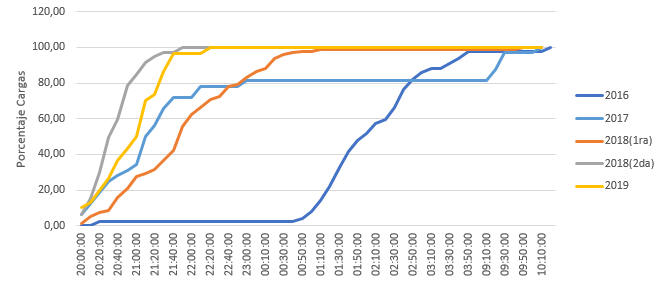
\includegraphics[width=\textwidth]{img/experienciasPorcCarga.png}
    \end{center}
  \caption{Porcentaje de carga}
  \label{graf:experienciaPorcCarga}
\end{figure}

A partir de estas experiencias podemos ver en la Figura \ref{graf:experienciaPorcCarga} el porcentaje acumulado durante el periodo de escrutinio para cada acto electoral.  \newline
En el año 2016, primer año que se utilizaba Gukena, se logró una buena velocidad de carga computando el 60\% de las mesas a las 22:30 hrs. Todo sistema nuevo requiere su periodo de aprendizaje y adaptación sobre los usuarios. Se puede comentar que en este año se cargaron algunas actas directamente por la Junta Electoral o la Secretaria cuando se recibían las urnas por distintas razones listadas en la subsección \ref{exp2016}. \newline
Analizando el tamaño del dominio, Gukena logró cubrir con éxito el proceso electoral en el 2018 cuando se requerían elegir todos los cargos de la UNComa y todos los claustros debían votar. Como se puede observar en el año 2018 (1ra vuelta) se logró una muy buena velocidad de carga logrando el 60\% del escrutinio luego de 2 horas de terminado el acto electoral.\newline
En la Figura \ref{graf:experienciaPorcCarga} se observa que el momento de mayor carga de cada año fluctúa entre las 20.30 y 23.00 hrs., notándose que por cada año nuevo que se utilizó Gukena se fue reduciendo el tiempo de espera para lograr la mayoría de las mesas cargadas. El sistema no modificó su integración dentro del proceso electoral por lo tanto, esta velocidad se logró por el aprendizaje de los usuarios. Sin necesidad de involucrar al sistema en la primer etapa del proceso, en la emisión del voto.

En la Figura \ref{graf:provincialConGukena} se muestra el porcentaje de carga de Gukena y las elecciones provinciales en Río Negro, Córdoba, Neuquén analizadas en la subsección \ref{analisisComparativoProvincial}.
Debido a que el horario del cierre del escrutinio a nivel provincial y en UNComa son distintos se debió modificar los tiempos de cargas de Gukena restándole 2 horas para que sean comparable entre ellas. Otra diferencia entre estas elecciones son la cantidad de mesas escrutadas, siendo mucho menor en UNComa, por lo tanto, se tomaron las experiencias de Gukena con mayor cantidad de mesas las cuales fueron las elecciones del 2018 (1ra y 2da vuelta). 


\begin{figure}[h!]
    \begin{center}
        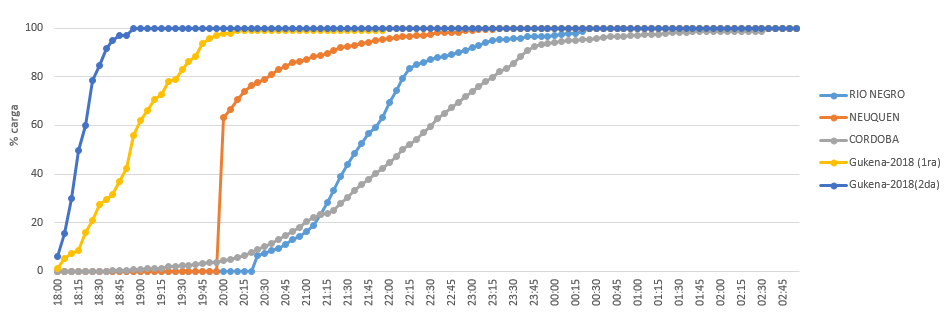
\includegraphics[width=\textwidth]{img/provincialGukena.png}
    \end{center}
  \caption{Porcentaje de carga comparativo}
  \label{graf:provincialConGukena}
\end{figure}

En la Figura \ref{graf:provincialConGukena} muestra distintos procesos electorales que involucran tecnología en diferentes etapas. En Rio Negro se involucró tecnología en la transmisión de resultados desde nodos zonales, manteniendo boletas partidarias en papel y escrutinio manual. Como variante a las elecciones de Río Negro, Córdoba sólo se diferencia en que utiliza la boleta única papel. Para ambas elecciones se puede ver que logra una curva constante y un crecimiento lento durante toda la noche de escrutinio. Por otro lado, las elecciones de Neuquén que utilizan tecnología en todo el proceso electoral muestran un pico de crecimiento a las 20:00 hrs. Finalmente, Gukena que utiliza tecnología en las etapas siguientes al escrutinio manual también consigue una buena velocidad de cómputos. Ambos logran en poco tiempo conseguir la mayoría de las mesas escrutadas disponibles en el sistema. Para esto ambos sistemas tuvieron que pasar por un aprendizaje por parte de los usuarios. En Gukena la cantidad de personas involucradas es menor que en el sistema BUE, ya que este último involucró capacitación tanto de los técnicos (mínimo uno por escuela), autoridades de mesa y de cada votante. Gukena sólo necesita la capacitación de una persona por mesa (Autoridad de Mesa), a quien se le envió un instructivo en papel incluido en el kit de la urna. Esta ventaja de Gukena reduce notablemente el presupuesto en capacitación con respecto al sistema BUE.

La encuesta de la opinión pública del sistema BUE, descrita en la subsección \ref{encuesta} nos dio evidencia de que los electores no tenían conocimiento del chip integrado en la boleta única electrónica y desconocían la existencia de la validación de estos chips usando la máquina. 
Además se pudo observar que las autoridades de mesa en muchos casos, dejan a las máquinas la responsabilidad del conteo usando el chip y no realizan un escrutinio manual para su validación.
Por lo tanto, se puede concluir que la curva del escrutinio en Neuquén es buena pero sin seguridad de que las máquinas realizaron un conteo correcto o que el chip integrado almacenó el dato correcto del votante. Gukena al no involucrarse en las etapas de emisión del voto y en el escrutinio de la mesa, logró una buena curva del escrutinio como en Neuquén, sin poner en riesgo la integridad del voto. 
